\documentclass[conference]{IEEEtran}
\IEEEoverridecommandlockouts

\usepackage{cite}
\usepackage{amsmath,amssymb,amsfonts,amsthm,mathtools}
\usepackage[alphabetic,backrefs,lite,nobysame]{amsrefs}
\usepackage{algorithm2e}
\usepackage{tikz-cd}
\usepackage{graphicx}
\usepackage{listings}
\usepackage{textcomp}
\usepackage{xcolor}
\usepackage{subcaption}
\newcommand{\red}[1]{\textcolor{red}{#1}}
\newcommand{\green}[1]{\textcolor{green}{#1}}
\newcommand{\gray}[1]{\textcolor{gray}{#1}}
\newcommand{\Edit}[1]{\textcolor{gray}{(#1)}}
\newcommand{\lp}{\operatorname{lp}}
\newcommand{\sh}{\operatorname{sh}}
\newcommand\pder[2][]{\ensuremath{\frac{\partial#1}{\partial#2}}} 
\newcommand{\R}{\mathbb{R}}
\newcommand\blfootnote[1]{%
	\begingroup
	\renewcommand\thefootnote{}\footnote{#1}%
	\addtocounter{footnote}{-1}%
	\endgroup
}

\DeclareMathOperator{\MSE}{MSE}
\DeclareMathOperator{\PD}{PD}
\DeclareMathOperator{\CONV}{conv}

\def\BibTeX{{\rm B\kern-.05em{\sc i\kern-.025em b}\kern-.08em
		T\kern-.1667em\lower.7ex\hbox{E}\kern-.125emX}}

\newtheorem{theorem}{Theorem}[section]
\newtheorem{conjecture}[theorem]{Conjecture}
\newtheorem{problem}[theorem]{Problem}
\newtheorem{prop}[theorem]{Proposition}
\newtheorem{cor}[theorem]{Corollary}
\newtheorem{corollary}[theorem]{Corollary}
\newtheorem{mr}[theorem]{Main Result}
\newtheorem{lemma}[theorem]{Lemma}
\newtheorem{claim}[theorem]{Claim}
\theoremstyle{definition}
\newtheorem{obs}[theorem]{Observation}
\newtheorem{definition}[theorem]{Definition}
\newtheorem{convention}[theorem]{Convention}
\numberwithin{figure}{section}
\newtheorem{remark}[theorem]{Remark}
\newtheorem{example}[theorem]{Example}
\newtheorem{algthm}[theorem]{Algorithm}

\graphicspath{{./img/}}

\begin{document}
	
	
	\title{Convolutional Persistence for Cubical Complexes
		\thanks{The  authors were partially supported by the Air Force Office of Scientific Research under the  grant ``Geometry and Topology for Data Analysis and Fusion",  AFOSR FA9550-18-1-0266.}
	}
	
	\author{
		Elchanan Solomon\\
		Department of Mathematics, \\
		Duke University\\
		Durham, USA \\
		yitzchak.solomon@duke.edu
		\and
		Paul Bendich\\
		Department of Mathematics, Duke University\\
		Geometric Data Analytics\\
		Durham, USA \\
		paul.bendich@duke.edu
	}
	
	\maketitle
	
	\begin{abstract}
		todo.
	\end{abstract}
	
\section{Overview}
Persistent homology is a method of assigning multiscale topological descriptors to parametric families of shapes. In \emph{functional} persistence, the object of study is a real-valued function $f:X \to \mathbb{R}$ defined over a space $X$, and the parametric family of shapes are the sublevel-sets $X_{\alpha} = \{x \in X : f(x) \leq \alpha\}$. It is similarly possible to consider superlevel-sets, which is equivalent to negating the \emph{filter function} $f$. One crucial feature of this construction is that $X_{\alpha}$ is a subset of $X_{\beta}$ for $\alpha \leq \beta$, so that the sublevel-sets are naturally nested. The output of persistent homology is a collection of intervals (equivalently, a collection of points), called a \emph{barcode} (or \emph{persistence diagram}, using the point representation). The space of barcodes is not a vector space, even approximately {\bf (cite!)}, but there do exist multiple \emph{vectorizations} that transform barcodes into vectors suitable for machine learning and data analysis.\\

A very general setting for functional persistence is that of \emph{cubical complexes}, i.e. shapes obtained by gluing together cubical regions like pixels or voxels. For example, if $X$ is a 2D rectangular grid, a function $f:X \to [0,1]$ can be viewed as a greyscale image. Persistent homology can then be understood as a feature extraction method for such images, either for supervised or unsupervised learning. Example applications include {\bf cite: removing image noise (Chung), parameter estimation for PDEs (Calcina, Adams), segmentation (Chen), flow estimation (Suzuki), tumor analysis (Crawford), cell immune micronenvironment (Carriere), and materials science (Hiraoka)}.\\

It should be understood that purely topological methods do not provide state-of-the-art predictive accuracy on most machine learning tasks, and are not to be considered as \emph{alternatives} to more general methods like neural nets and kernel methods. Rather, topological methods provide \emph{principled} and \emph{intepretable} features that are different from those extracted by other methods, and can help improve the performance and utility of the entire pipeline.

To that end, it is important to understand the properties of functional persistence and their role in machine learning. Here we consider some of the most salient features:
\begin{itemize}
	\item (Computational complexity) For a cubical complex $K$ with $N$ cubes, computing persistence is $O(N^\omega)$, where $\omega$ is the matrix multiplication constant. This means that such persistence calculations scale poorly in the resolution of data, especially high-dimensional data, where doubling the resolution in $\mathbb{R}^d$ results in a $2^{d}$-fold increase in the number of simplices.
	\item (Stability) Persistent homology is stable to small perturbations of the input data, in that the distance between the barcodes for two functions $f$ and $g$ on a common space $X$ is bounded by $\|f-g\|_{\infty}$. However, persistence is not stable to outliers, so images that look similar outside of a small fraction of pixels can produce wildly different barcodes.
	\item (Flexibility) There is a single persistence diagram to be associated with each pair $(X,f)$ of space $X$ and real-valued function $f$. This lack of additional parameters makes applying persistence straightforward, but can also be limiting in contexts where featurizations should be data-dependent. 
	\item (Invertibility) There exist many space-function pairs $(X,f)$ and $(Y,g)$ producing identical barcodes. Thus, persistence is not invertible as feature map, and this loss of information may hinder the capacity of persistence-based methods to identify patterns or distinguish distinct images.
\end{itemize}

Our goal in this paper is to introduce a modification to persistence of cubical complexes that is (1) faster to compute, (2) more stable to outliers, (3) allows for data-driven tuning, and (4) is provably invertible. Essentially, this technique consists of passing multiple convolutional filters over an image and computing the persistence of the resulting collection of low-resolution outputs. Since this pipeline consists principally of combining convolutions with persistence, we call it \emph{convolutional persistence}.

The remainder of the paper is organized as follows. Section II provides a thorough, non-technical survey on persistent homology. Section III reviews related work, and places \emph{convolutional persistence} in conversation with prior work on inverse problems in computational topology. Section IV contains the major theoretical results of the paper, with the highlight being {\bf Theorem ?} proving injectivity for convolutional persistence. Section V compares ordinary and convolutional persistence on a host of datasets, showing the capacity of convolutional persistence to produce features well-suited for image classification. Finally, Section VI discusses outstanding questions and generalizations of this work.

\section{Background}
\label{sec:background}
The content of this paper assumes familiarity with the concepts and tools of persistent homology. Interested readers can consult the articles of Carlsson \cite{carlsson2009topology} and Ghrist \cite{ghrist2008barcodes} and the textbooks of 
Edelsbrunner and Harer \cite{edelsbrunner2010computational} and Oudot \cite{oudot2015persistence}. We include the following primer for readers interested in a high-level, non-technical summary.

\subsection{Persistent Homology}

Persistent homology records the way topology evolves in a parametrized sequence of spaces. In the case of functional persistence, we consider an ambient space $X$ filtered by a real-valued function $f:X \to \mathbb{R}$. When $X$ is a cubical complex, made by gluing together cubes of varying dimension (vertices, edges, squares, cubes, etc.), this construction is particularly simple. To every cube $\sigma$ we associate a real value $f(\sigma)$ that encodes the time at which it appears in the filtration of $X$. The only restriction on the function $f$ is the following consistency condition: if $\sigma$ is a sub-cube of a higher-dimensional cube $\tau$ (i.e. an edge which sits at the boundary of a square), we must have $f(\sigma) \leq f(\tau)$, ensuring that cubes do not appear before any of their faces.\\


Given a filtered cubical complex, as the sequence of sublevel-sets evolves, the addition of certain edges or higher-dimensional simplices alters the \emph{topological type} of the space. A precise way of quantifying topology is \emph{homology}, which measures the number of connected components (zero-dimensional homology), cycles (one-dimensional homology), or voids (higher-dimensional homology) in a space. Thus, homology can change when two connected components merge or a new cycle is formed. Simplices responsible for such topological changes are called \emph{critical}. Persistent homology records the parameter values at which critical simplices appear, notes the dimension in which the homology changes, and pairs critical values by matching the critical value at which a new homological feature appears to the critical value at which it disappears. This information is then organized into a structure called a \emph{barcode}, which is simply a collection of intervals. Figure \ref{fig:cubpers} shows the computation of the zero- and one-dimensional barcodes for a simple cubical complex.\\

\begin{figure}
	\centering
	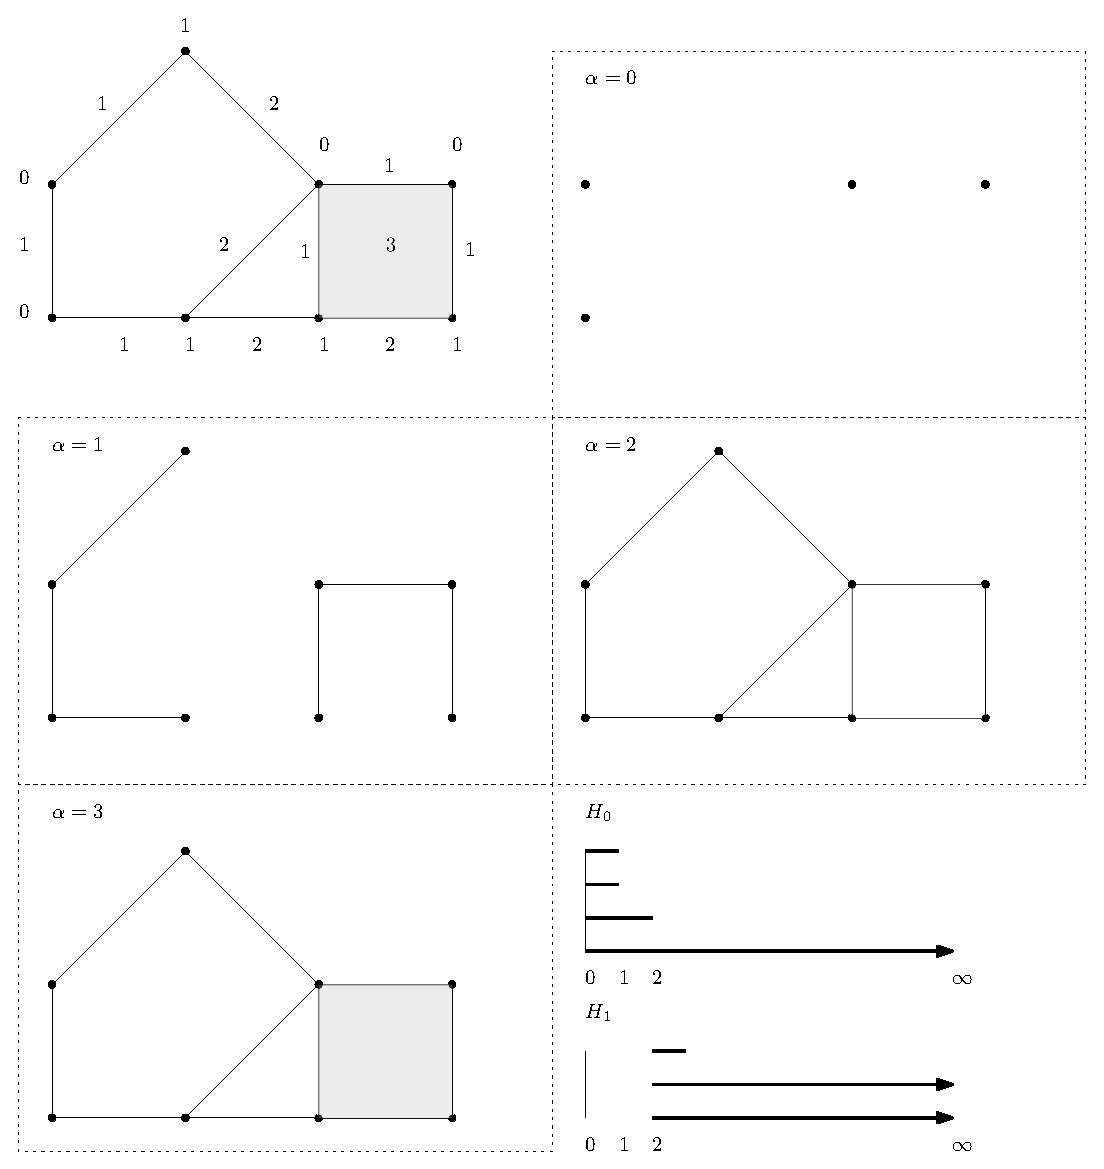
\includegraphics[scale=0.5]{cubpers.eps}
	\caption{Top-left: A cubical complex with filtration values attached to vertices, edges, and squares. Top-right through bottom-left: sublevel-sets associated with different threshold values. Bottom-right: barcodes in dimensions zero and one. The zero-dimensional homology $H_0$ barcode contains four bars, since at $\alpha=0$ there are four connected components. Two bars die at $\alpha=1$, since at that threshold value there are only two connected components. Finally, $\alpha=2$ sees the merger of these connected component, so another bar dies at $\alpha=2$ and the last persists to infinity. In one-dimensional homology $H_1$, three bars are born at $\alpha = 2$, when three loops appear in the sublevel-set, and one of these bars dies at $\alpha=3$, when that loop is killed off by the introduction of a square.}
	\label{fig:cubpers}
\end{figure}

When working with cubical complexes, it is possible to limit the maximal dimension of simplices allowed in the construction. Given an arbitrary cubical complex $K$, we write $K^m$ to denote the subcomplex consisting of all cubes of dimension at most $m$; this is called the \emph{$m$-skeleton of $K$}. Note that $K$ and $K^m$ have the same homology in dimensions less than $m$, but may differ in dimension $m$, and $K^m$ has no homology in dimension greater than $m$.

\subsection{Image Cubical Complexes}
Given a $d$-dimensional grayscale image, there are two ways of turning this data into a cubical complex. One is to view the voxels as being vertices, and higher-dimensional cubes as coming from voxels adjacencies, so that pairs of adjacent pixels form an edge and squares come from four voxels in a square formation, etc. There is a canonical way of extending the function $f$ from the voxels (vertices) to the entire complex: given a cube $\tau$, define $f(\tau)$ to be $\max_{\sigma} f(\sigma)$, where the max is taken over all vertices $\sigma < \tau$. Thus, a square appears precisely once all its constituent vertices appear; this is called the \emph{lower-*} filtration.\\

Alternatively, one can also view the voxels as being $d$-dimensional cubes, and have the lower-dimensional cubes be the faces of these vertices. As before, there is a canonical way of extending the function value from the voxels (top-dimensional cubes) down to entire complex: for a cube $\sigma$, define $f(\sigma)$ to be $\min_{\tau} f(\tau)$, where the min is taken over all voxels $\tau$ that contain $\sigma$. Thus, a cube appears precisely when at least one of the voxels in which it participates does;  this is called the \emph{upper-*} filtration.\\ 

Consult figure \ref{fig:image_to_complex} for an illustration of these two images complexes. Generally, these complexes will differ, and the resulting persistence barcodes will be different. However, there exists a formula for reading the barcodes for one construction from the barcodes of the other, see \cite{bleile2021persistent}. In this paper, we will adopt the former construction, taking our voxels to be the vertices of the cubical complex. {\bf Is this what GIOTTO does?}


\begin{figure}
	\centering
	
\includegraphics[scale=2]{image_to_complex.eps}
	\caption{A $2 \times 2$ image can be turned into a complex in one of two ways. Left: A complex with four top-dimensional cubes, with function values, indicated using color, extended to vertices and edges via the lower-* rule. Right: A complex with four vertices, with function values extended to the edges and interior square via the lower-* rule.}
	\label{fig:image_to_complex}
\end{figure}
\subsection{Comparing Persistence Diagrams}

As multi-sets of points in the plane, persistence diagrams are not vectors. However, there exist multiple metrics for comparing persistence diagrams. The most common approach is to view persistence diagrams as discrete distributions on the plane $\mathbb{R}^2$, and use techniques from optimal transport theory, such as $p$-Wasserstein metrics $W_p$, to compare them. This analogy is complicated by the fact that persistence diagrams do not all have the same number of points, and that points in a persistence diagram near the diagonal line $y=x$ correspond to transient homological features, dying shortly after they are born, which ought not to play an important role in dictating similarity of diagrams. These problems are ameliorated by modifying the optimal transport protocol to allow paring points in one diagram either with points in the other diagram or with the diagonal line $y=x$, the latter incurring a cost proportional to the distance of the given point from the diagonal. This \emph{diagonal paring} allows us to define an optimal transport distance between any pair of diagrams, regardless of how many points they have. In practice, the $p$-Wasserstein metrics in use are either $p=1,p=2$, or $p=\infty$, the latter of which is called the \emph{Bottleneck distance} in persistence theory, and is written $d_B$. See Figure \ref{fig:wasserstein} for a visualization of a matching between persistence diagrams.  

\begin{figure}
	\centering
	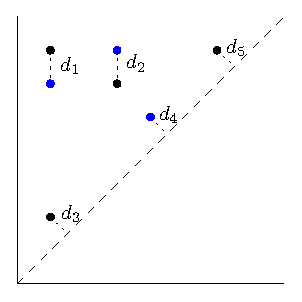
\includegraphics[scale=1]{wasserstein.eps}
	\caption{Two persistence diagram $D_1$ and $D_2$, one in black and the other in blue. An optimal matching between these diagrams is shown, containing both diagonal and non-diagonal pairings. The resulting $p$-Wasserstein distance is then $W_{p}(D_1,D_2) = \sqrt[p]{d_1^p + d_2^p + d_3^p + d_4^p + d_5^p}$.}
	\label{fig:wasserstein}
\end{figure}


\subsection{Computational Complexity}
Persistence calculations are $O(N^{\omega})$, where $N$ is the number of simplices in the filtration and $\omega$ is the matrix multiplication constant \cite{milosavljevic2011zigzag}. For a metric space $X$, the number of $(d+1)$-dimensional simplices in the Rips complex is ${|X| \choose d+2}$, which are needed for computing persistence in degree $d$. Thus the computational complexity of $d$-dimensional Rips persistence is $O({|X| \choose d+2}^{\omega})$, which is huge even for small values of $d$. Though this bound is in practice quite pessimistic, it is accurate in reflecting the poor scaling of persistence calculations in $|X|$ \cite{otter2017roadmap}.

The bottleneck distance between persistence diagrams can be computed exactly using the well-known Hungarian algorithm, whose complexity is $O(n^3)$ for pairs of diagrams with at most $n$ points. The number of points in the persistence diagram of filtration is always bounded by the total number $N$ of simplices in the filtration, and may be much smaller. If one is interested in \emph{approximating} the bottleneck, or more generally, $p$-Wasserstein distances between persistence diagrams, there are significantly faster methods than the Hungarian algorithm. One such method is based on \emph{entropic approximation} techniques from optimal transport \cite{lacombe2018large}, and provided that the norms of the points in the diagrams are uniformly bounded by some constant $C$, a transport plan within $\epsilon$ of the optimal matching can be produced in $O(\frac{n \log(n) C}{\epsilon^2})$ iterations of the Sinkhorn algorithm, which is itself linear in $n$. This algorithm is implemented in the persistent homology library GUDHI that we use in our experiments, and hence the computational complexity of our framework as a whole is dominated by the calculation of the diagrams themselves, and not the $p$-Wasserstein distances between them.

\subsection{Properties of Persistent Homology}
\label{subsec:persprop}
Persistence theory guarantees that a small modification to the filtration of a metric space produces only small changes in its persistence diagram. To be precise, if the appearance time of any given simplex is not delayed or advanced by more than $\delta$, the persistence diagram as a whole is not moved by more than $\delta$ in the Bottleneck distance \cite{cohen2007stability}. This implies that a small error in distance measurements in $X$ produces only small distortion in the resulting persistence diagram. However, persistent homology is not at all stable to \emph{outliers}, i.e. a small subset of the data having large error \cite{buchet2014topological}. 

Another important feature of persistent homology is that the pipeline mapping a metric space to a persistence diagram is \emph{almost everywhere differentiable}  \cite{gameiro2016continuation,poulenard2018topological}. This is because the coordinates of the points in the diagram correspond locally to fixed critical simplices in the data. In the Rips complex, all such simplices are edges; to increase or decrease a diagram coordinate value, one increases or decreases the length of the corresponding edge by pushing its two boundary points either further together or closer apart. To extend the example of Figure \ref{fig:filtration}, consider what would happen if the right-most point were dragged further to the right: this would delay the creation of the larger cycle, and the corresponding point in the persistence diagram would go from $(2,\cdot)$ to $(2+\delta,\cdot)$.
The pairing of critical edges with coordinates in the diagram is well-defined locally, but non-infinitesimal perturbations of the metric space tend to shuffle around the critical pairings and change which edges are critical. There are also degenerate situations in which the pairing of edges with coordinate values in the diagram is not uniquely defined -- these cases can be addressed theoretically, but do not concern us here as they are a measure-zero phenomenon. This differentiability of persistent homology allows us to use gradient descent methods for topological optimization  \cite{carriere2021optimizing}.  


It is also important to note that persistent homology is not an injective invariant of metric spaces, meaning that different spaces can have the same persistence diagrams \cite{curry2018fiber,leygonie2021fiber,leygonie2021algorithmic}. Thus, some information is lost in the process of converting a metric space to a persistence diagram.


Our focus in this paper is the task of computing functional sublevelset persistence. This is a very general invariant that can be computed for \emph{constructible functions} on \emph{definable sets}, which includes monotonic functions on simplicial complexes. However, we specialize here to the simple, ubiquitous setting where the domain is a cubical grid. This is not strictly necessary for the theory developed here, but significantly simplifies the analysis and computational pipeline, and encompasses many of the applications of interest.\\

To be precise, let $P \subset \mathbb{Z}^d$ be a rectangle inside of the integer lattice, and let $f: P \to \mathbb{R}$ be a function defined on $P$. $P$ can be viewed as the vertex set of an $m$-dimensional cubical complex $K^{m}_{P}$ in which higher-dimensional simplices are given by grid adjacencies, and $f$ can be extended to this complex via the lower-* rule, in which $f(\sigma) = \max_{p \in \sigma}f(p)$, cf. \cite{bleile2021persistent} section 4. Taking the \emph{maximum} here guarantees that a simplex does not appear in a sublevelset filtration until all of its faces do, ensuring that the sublevelsets are valid subcomplexes.\\

There are many areas of application in which the topology of the pair $(K^{m}_{P},f)$ is useful. However, there are multiple challenges with computing and using these persistence diagrams:
\begin{itemize}
	\item Persistent homology calculations scale poorly in the size of the input complexes, and hence cannot be effectively applied to many high-resolution images.
	\item Persistent homology calculations are sensitive to outliers, and many real-world images exhibit considerable noise.
	\item Even in the absence of noise, the topological structure in an image may not be evident without some image preprocessing.
	\item Different forms of preprocessing will produce different topological structures in the resultant image. How should we decide which is most relevant for the task at hand?
	\item Functional persistence is not injective, so different images can have the same persistence diagram. This implies a loss of information in any framework that makes decisions on the basis of these diagrams.
\end{itemize}

In this paper, we propose a framework for computing persistence of pairs $(K^{m}_{P},f)$ that addresses all of these concerns simultaneously. This framework is adapted from the concept of a \emph{convolution layer} in modern deep learning. Let $B \subset \mathbb{Z}^d$ be another rectangle, smaller than $P$, and let $g: B \to \mathbb{R}$ be a function on this region; the pair $(B,g)$ acts as a \emph{convolutional filter}. Fix a vector $k = (k_1, \cdots, k_d)$ with $k_i \in \mathbb{N}_{>0}$, corresponding to the \emph{stride} of the convolution. For $v \in \mathbb{Z}^d$, define:
\[(g \ast f)(v) = \sum_{p \in B} g(p)f(p+v \odot k),\]

where $\odot$ is the Hadamard product.Let $R \subset \mathbb{Z}^d$ be the collection of values $r$ such that $B + (r \cdot k) \subseteq P$, which is necessarily also a rectangle. The pair $(R, g \ast f)$ is the output of our convolution. $R$ may be much smaller than the support of $f$, since the various translates of $B$ covering this support are not required to overlap much, if at all. In the degenerate setting where $P$ and $B$ are the same shape, $R$ will consist of a single vertex. For the purposes of computing persistence, we will think of $R$, like $P$, as being the vertex set of a cubical complex $K_{R}^{m}$, and we extend functions on $R$ to the entirety of the cubical complex using the lower-* rule.\\

By analogy with \cite{solomon2021fast,solomon2021geometry}, we propose that the collection of persistence diagrams of the form $PH(K_{R}^{m},g_{i} \ast f)$, for some set of filter functions $\mathcal{G} = \{g_i\}$, is of greater general utility than $PH(K_{P}^{m},f)$. The computational advantages are immediate: when the stride $k$ is large, so that $R$ is much smaller than $P$, we have replaced a single, very expensive calculation with multiple, significantly faster calculations that can be performed in parallel. Moreover, we claim that this approach, which we deem \emph{convolutional persistence}, is more robust and flexible than ordinary persistence, and has superior inverse properties. It is also important to note that the \emph{translation equivariance} of convolutions and the \emph{transational invariance} of persistent homology work well together.\\

%It is also important to note that convolution is \emph{translation equivariant} and persistence is \emph{translation invariant}, so their composition is translation invariant.\\

\emph{Stability and robustness} are not hard to justify. If $g$ is a filter function with $\|g\| \leq 1$, then $\|g \ast f_1 - g \ast f_2 \| \leq \|f_1 - f_2\|$ by the Cauchy-Schwarz inequality, providing stability. A classical example is the \emph{box-smoothing} filter $g(p) = \frac{1}{|B|}$. Such smoothing filters also do a good job of diminishing the impact of outliers. \emph{Flexibility} is also immediate, since the collection of filters $\mathcal{G}$ can be curated for the task at hand, and can be learned using a training dataset.\\

Let us now demonstrate injectivity. For a fixed function $f:P \to \mathbb{R}$ and stride vector $k$, we can obtain a mapping $\iota_{f}$ of the rectangle $R$ into $\mathbb{R}^{|B|}$ by sending every point $r \in R$ to the vector $\{f(b + k \odot r) \mid b \in B\}$. This is technically a set, rather than a vector, but it becomes a vector after fixing an order on the elements of $B$. Such a mapping can be extended linearly to the entire cubical complex $K_{R}$ built on top of $R$. Let us suppose that $\iota_{f}$ is injective on the $m$-skeleton $K_{R}^m$, so that $\iota_{f}(K_{R}^m)$ has the structure of a simplicial complex isomorphic to $K_{R}^m$. Then for a function $g: B \to \mathbb{R}$, viewed also as a vector $\vec{g} \in \mathbb{R}^{|B|}$, and threshold value $t$, the sets $\{\sigma \in K_{R}^{m} \mid g(\sigma) \leq t\}$ and $\{\sigma \in \iota_{f}(K_{R}^m) \mid \sigma \cdot \vec{g} \leq t \}$ are homeomorphic. See Figure \ref{fig:embedding} for a visual schematic. This means that the persistence diagram $PH(K_{R}^m,g \ast f)$ is identical to the persistence diagram $PH(\iota_{f}(K_{R}^m),\langle g, \cdot \rangle)$. If $g$ is varied over the unit sphere in $\mathbb{R}^{|B|}$, the set of diagrams $PH(\iota_{f}(K_{R}^m),\langle g, \cdot \rangle)$ is known as the \emph{Persistent Homology Transform} which is known to be injective, see \cite{turner2014persistent,ghrist2018persistent,curry2018many}. Thus, the collection of persistence diagrams of the form $\{PH(K_{R}^m, g \ast f) \mid g : B \to \mathbb{R}\}$ is injective. Note that the distinction between using all functions $g: B \to \mathbb{R}$, or only normalized functions lying on the sphere, is immaterial, as persistent homology transforms trivially under rescaling of the height function, so these two invariants determine one another.\\ 

%\marginnote{\footnotesize \color{red} Cite PHT papers}
\begin{figure}
	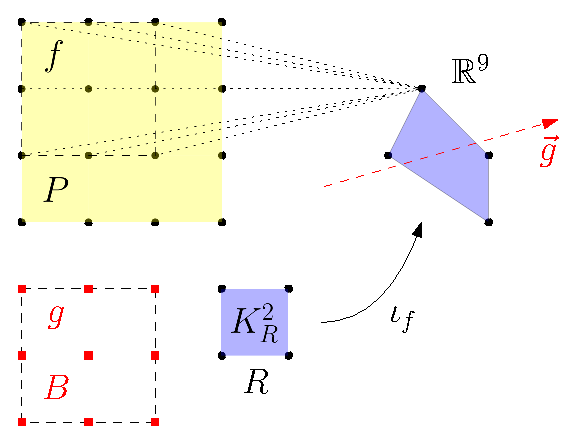
\includegraphics{embedding}
	\caption{The function $f$ is defined on the $4 \times 4$ grid on the top left. The box $B$ is $3 \times 3$, and using a $(1,1)$-stride there are four ways of laying $B$ over the domain of $f$, so that $R$ is a $2 \times 2$ grid. We can map the vertices of $R$ into $\mathbb{R}^9$ by associating each vertex of $R$ with its corresponding translate of $B$, and then taking as coordinates the values of $f$ in that translate. This extends linearly to a map $\iota_{f}$ from the complex $K_{R}^2$ in $\mathbb{R}^9$, which here is shown to be an embedding.}
	\label{fig:embedding}
\end{figure}

The above proof of injectivity for \emph{convolutional persistence} relies on $\iota_{f}:K_{R}^{m} \to \mathbb{R}^{|B|}$ being injective. We claim that this is generically the case whenever $\kappa = \Pi_{i}k_i > 2m$. Indeed, let $B^{*} \subseteq B$ consist of those elements in the top-left $k_1 \times k_2 \times \cdots k_d$ corner of $B$. The various translates $B^{*} + (k \odot r)$ are all disjoint subsets of $P$. We can thus view the vertices $\{f(b + k \odot r) \mid b \in B\}$ of $\iota_{f}(K_{R}^m)$ as having at least $\kappa$ degrees of freedom, and this can be made more precise by projecting the embedding on to the coordinates corresponding to $B^*$. We now want to show that if we choose a collection $S$ of points in $\mathbb{R}^{M}$ for $M > 2m$, and build the complete $m$-dimensional complex on top of these points, we will generically never have nontrivial intersections of disjoint simplices. To see why this is the case, let $\sigma$ and $\tau$ be simplices corresponding to disjoint subsets $S_{\sigma}$ and $S_{\tau}$ of $S$. If $\sigma$ and $\tau$ intersect, then their union is contained in an affine subset of $\mathbb{R}^M$ of dimension $(\dim \sigma + \dim \tau)$. Now, whenever $M > \dim \sigma + \dim \tau$, a collection of at least $(\dim \sigma + \dim \tau + 2)$ points generically does not lie on an affine subset of dimension $(\dim \sigma + \dim \tau)$. Since $M > 2m \geq \dim \sigma + \dim \tau$, and $|S_{\sigma} \cup S_{\tau}| = |S_{\sigma}| + |S_{\tau}| = (\dim \sigma + 1) + (\dim \tau + 1) = \dim \sigma + \dim \tau + 2$, we see that the intersection of $\sigma$ and $\tau$ is not generic.\\

What we have just shown is that having a large stride vector, in addition to providing computational speedups by lowering the resolution of the resultant grid, also provides generic injectivity for persistence of higher-dimensional data complexes.\\ 

Now, what we have described above is persistence with a single convolutional layer. One can extend this construction by convolving the collection $\{(R, f \ast g) \mid g \in \mathcal{G}\}$ using a new rectangle $B'$ and collection $\mathcal{H}$ of filter functions $h: B' \to \mathbb{R}$, and \emph{then} compute persistence. This pipeline remains injective, because the collection $\{(R, g \ast f) \mid g: B \to \mathbb{R}\}$ determines the function $f$ (this is trivial, consider characteristic functions of pixels in $B$), so the two-layer convolutional persistence is a composition of two injective operations, where we are now taking the sets $\mathcal{G}$ and $\mathcal{H}$ to consist of \emph{all possible filters}. We might also consider introducing a non-linear activation between the convolutional layers, following more closely the structure of a CNN.\\

An alternative convolutional pipeline is to do a convolutional with a small stride, so that the resulting image has the same resolution as the original, and then apply a pooling later. This mirrors more closely the structure of a modern CNN. Note that this pipeline also enjoys an inverse result, provided that the corresponding embedding is injective on the input cubical complex.\\

In practice, of course, we are not interested in considering infinitely many filter functions. Indeed, learning tasks require invariants to \emph{retain} features that are important to classification or regression, and \emph{forget} features that are not. Thus, we will want to pick $\mathcal{G}$ appropriately. There are many ways for this choice to be made:
\begin{enumerate}
	\item Take $\mathcal{G}$ to consist of a collection of popular filters in image processing, like blurring, sharpening, and boundary detection.
	\item Take $\mathcal{G}$ to consist of Klein filters, as identified by Carlsson et al.
	\item Take $\mathcal{G}$ to consist of eigenfilters identified via PCA on the set of patches of images in the training set.
	\item Incorporate convolutional persistence in a deep learning pipeline and learn $\mathcal{G}$ to minimize a chosen loss function.
\end{enumerate}

For the third point above, note that the inverse results for the PHT do not require all sphere directions when the shape in question sits inside a low-dimensional space of Euclidean space. Thus, it makes sense to ignore filters orthogonal to the space of image patches in question.\\

%and this introduces an important tradeoff in convolutional optimization. When the convolutional rectangle $R$ and the stride $k$ are large, the decrease is resolution is quite substantial, yet the number of free parameters to be learned is large. This makes optimization difficult, but also allows for more sophisticated filters. Conversely, when the rectangle and stride are small, there is a more minor decrease in resolution, but a simpler optimization task. As for learning more complicated filters, this is still possible when there are multiple convolutional layers.\\ 
 
  
{\bf Prior Work:} This is not the first work where convolutions and persistence have been investigated. They were considered in APE I. They are also mentioned in ``PLLay: Efficient Topological Layer based on Persistence Landscapes". What makes this work unique is that it extends APE I by considering general convolutional layers, rather than noisy box smoothing, and it extends the PPLay paper by considering non-deep-learning approaches to convolutional persistence, focusing on the ability of convolutionals to speed up persistence calculations, rather than just extract more features for a CNN, and investigating more deeply into questions of injectivity and optimization.\\

{\bf Goal:} The goal of this paper is to verify or rule out the following conjectures: 
\begin{itemize}
	\item Convolutional persistence can achieve reasonable accuracy on complex learning tasks for shapes defined by height functions over cubical grids.
	\item Convolutional persistence can be incorporated into other deep learning pipelines and provide some improvement in accuracy.
\end{itemize}


{\bf Experimental Pipeline:}
\begin{enumerate}
	\item In the first phase of the pipeline, we consider the digits dataset, which is small enough that ordinary persistence calculations are very fast. Thus, the role of this phase is to understand how convolutions improve the utility of persistence features. The first step of this phase is to see how standard ML models perform on digit classification based on cubical persistence features. We can then enrich this featurization using different choices of fixed filters $\mathcal{G}$, as outlined above, and see the impact this has on performance. The fundamental question here is whether or not reasonably good performance can be achieved through convolutional persistence. 
	\item The second phase of the pipeline is to try and learn the filters $\mathcal{G}$ using a deep learning architecture. This will require more work than choosing fixed filters as above.
	\item The third phase is to extend the experiments above to larger data sets, like CIFAR, where the downsampling aspect of the convolutions will also be of importance.
\end{enumerate}


\bibliography{convpersbib}
%
%
%$K$ be a pure $d$-dimensional simplicial complex, meaning that every simplex in $K$ is the face of some $d$-simplex. Let $f: K \to \mathbb{R}$ be a function on the top-dimensional simplices of $K$ extended to all of $K$ via the upper-* filtration: $f(\sigma) = \min \{f(\tau) \mid \sigma < \tau \mbox{ and } \operatorname{dim}(\tau) = d\}$. A very general example is when $K$ is a finite grid complex in $\mathbb{R}^d$, and $f:K \to \mathbb{R}$ records the values of some image defined on the pixels or voxels of $K$.


%a \emph{cubical complex} $K$ arising as the intersection of the integer grid complex $\mathbb{Z}^d$ in $\mathbb{R}^d$ with a rectangle of the form $\Pi_{i=1}^{d}[a_i,b_i]$, where $a_i, b_i \in \mathbb{Z}$. We will call such a complex $K$ a \emph{finite integer grid}. Given a real-valued function $f$ on the $d$-dimensional cells of $K$, this naturally extends to all of $K$ by asserting that $f(\sigma) = \min \{f(\tau) \mid \sigma < \tau \mbox{ and } \operatorname{dim}(\tau) = d\}$. When $d=2$, such a pair $(K,f)$ is simply an image defined over a rectangular array of pixels, and for $d=3$ we have an image defined over a rectangular array of voxels. More generally, we might allow $f$ to take values in $\mathbb{R}^k$ for $k>1$, in which case we have an image with multiple \emph{channels}.\\

%That is, we consider covering $K$ with translates of a fixed subgrid $L$, and denote the dual of the \v{Cech} complex of the cover by $K/L$. If, moreover, we equip $L$ with a function $g: L \to \mathbb{R}$, we have a recipe for producing a function on the top-dimensional cells of $K/L$, which works as follows: Let $U \subset K$ be a set in the cover of $K$ by translates of $L$, which gives rise to a top-dimensional simplex $[U]$ in $K/L$, and define $f \ast g$ on $[U]$ to be $\sum_{\tau \in U} f(\tau)g(\tau)$, where the sum is taken over $d$-dimensional simplices in $U$.  




\end{document}